\begin{center}
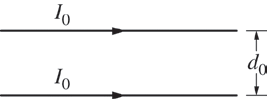
\includegraphics[scale=0.5]{images/img-005-015.png}
\end{center}

% Multiple Choice Question 17
\begin{questions}\setcounter{question}{16}\question
Two long, straight wires are fixed parallel to one another a distance $d_{0}$ apart. The wires carry equal constant currents $I_{0}$ in the same direction. The attractive magnetic force per unit length between them is $f=F / L$. What is the force per unit length between the wires if their separation is $2 d_{0}$ and each carries current $2 I_{0}$ ?

\begin{oneparchoices}
\choice $f / 4$
\choice $f / 2$
\choice $f$
\choice $3 f / 2$
\choice $2 f$
\end{oneparchoices}\end{questions}

